\documentclass[tikz,border=5pt]{standalone}
\usepackage{amssymb,amsmath}
\usetikzlibrary{arrows.meta,calc,decorations.pathreplacing}

\begin{document}
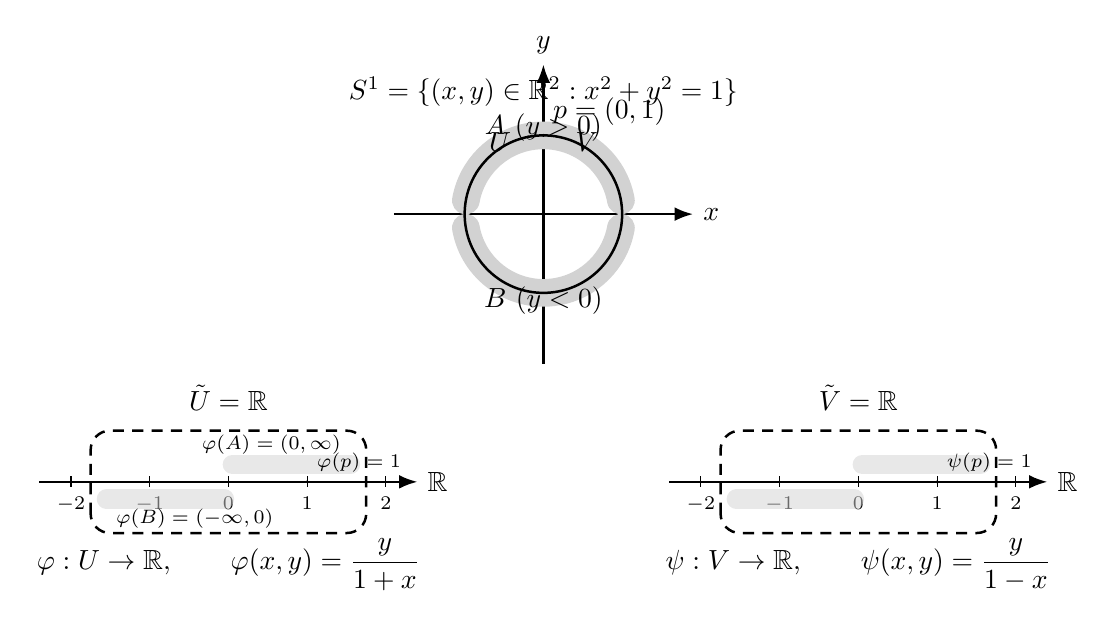
\begin{tikzpicture}[>=Latex,scale=1]

% ----------------------------
% Styles
% ----------------------------
\tikzset{
	s1/.style={line width=0.9pt},
	coverU/.style={line width=1.0pt,dashed,dash pattern=on 4pt off 3pt},
	coverV/.style={line width=1.0pt,dashed,dash pattern=on 4pt off 3pt},
	overlap/.style={line width=10pt,draw=gray!35,line cap=round},
	hole/.style={fill=white,draw=black,line width=0.7pt,dashed},
	maparr/.style={->,line width=0.9pt},
	trans/.style={->,line width=0.9pt},
	axis/.style={->,line width=0.8pt},
	dom/.style={draw=black,dashed,dash pattern=on 4pt off 3pt,line width=0.9pt,rounded corners=7pt},
	grayseg/.style={line width=7pt,draw=gray!35,line cap=round,opacity=.5}
}

% ============================================================
% TOP: S^1 \subset R^2 with concrete coordinates
% ============================================================
\begin{scope}[shift={(0,3.4)}]
	\def\r{1}
	
	% Coordinate axes in R^2 (optional; comment out if you want a cleaner look)
	\draw[axis] (-1.9,0) -- (1.9,0) node[right] {$x$};
	\draw[axis] (0,-1.9) -- (0,1.9) node[above] {$y$};
	
	% S^1
%	\draw[s1] (0,0) circle (\r);
	
%	% Mark the points (-1,0), (1,0) (on radius \r circle)
%	\coordinate (mone) at (-\r,0); % (-1,0) on the drawn circle
%	\coordinate (pone) at ( \r,0); % ( 1,0) on the drawn circle
%	
%	\node[below left]  at (mone) {$(-1,0)$};
%	\node[below right] at (pone) {$(1,0)$};
%	
%	% "Remove" them (white holes)
%	\draw[hole] (mone) circle (0.1);
%	\draw[hole] (pone) circle (0.1);
	
%	% U = S^1 \ {(-1,0)} : dashed circle with a small gap at angle 180°
%	\draw[coverU] (175:\r) arc (175:360:\r);
%	\draw[coverU] (0:\r)   arc (0:5:\r);
	
%	% V = S^1 \ {(1,0)} : dashed circle with a small gap at angle 0°
%	\draw[coverV] (5:\r)    arc (5:180:\r);
%	\draw[coverV] (180:\r)  arc (180:355:\r);
	
	% U \cap V = S^1 \ {(-1,0),(1,0)} = A \sqcup B (upper/lower arcs), shaded
	\draw[overlap] (10:\r)  arc (10:170:\r);   % A (upper, y>0)
	\draw[overlap] (190:\r) arc (190:350:\r);  % B (lower, y<0)
	
	% Re-draw boundary for crispness
	\draw[s1] (0,0) circle (\r);
	
	% Labels U,V,A,B
	\node at (-0.55,0.92) {$U$};
	\node at ( 0.55,0.92) {$V$};
	\node at (0, 1.10) {$A\ (y>0)$};
	\node at (0,-1.10) {$B\ (y<0)$};
	\node at (0,1.55) {$S^1=\{(x,y)\in\mathbb{R}^2:x^2+y^2=1\}$};
	
	% Anchors for downward arrows
	\coordinate (uAnchor) at (-0.60,-0.45);
	\coordinate (vAnchor) at ( 0.60,-0.45);
	
	% A sample point p=(0,1) on the circle (top)
	\coordinate (p) at (0,\r);
	\fill (p) circle (0.02);
	\node[above right] at (p) {$p=(0,1)$};
\end{scope}

% ============================================================
% BOTTOM LEFT: chart (\tilde U, \varphi) with concrete formula
% stereographic projection from (-1,0):
%   \varphi(x,y)= y/(1+x)
% ============================================================
\begin{scope}[shift={(-4.0,0)}]
	% Real line axis
	\draw[axis] (-2.4,0) -- (2.4,0) node[right] {$\mathbb{R}$};
	
	% Dashed "chart box" (purely schematic)
	\draw[dom] (-1.75,-0.65) rectangle (1.75,0.65);
	\node[above] at (0,0.78) {$\tilde U=\mathbb{R}$};
	
	% Tick marks
	\foreach \t in {-2,-1,0,1,2}{
		\draw (\t,0.07) -- (\t,-0.07);
		\node[below] at (\t,-0.07) {\scriptsize $\t$};
	}
	
	% Images of A and B under \varphi:
	% A (y>0) -> (0,\infty),  B (y<0) -> (-\infty,0)
	\draw[grayseg] (0.05, 0.22) -- (1.55, 0.22);
	\draw[grayseg] (-1.55,-0.22) -- (-0.05,-0.22);
	
	\node at (0, -1.05) {$\displaystyle \varphi:U\to\mathbb{R},\qquad
		\varphi(x,y)=\frac{y}{1+x}$};
	\node[above left] at (1.55,0.22) {\scriptsize $\varphi(A)=(0,\infty)$};
	\node[below right] at (-1.55,-0.22) {\scriptsize $\varphi(B)=(-\infty,0)$};
	
	% Image of p=(0,1):  \varphi(0,1)=1
	\fill (1,0) circle (0.02);
	\node[above right] at (1,0) {\scriptsize $\varphi(p)=1$};
\end{scope}

% ============================================================
% BOTTOM RIGHT: chart (\tilde V, \psi) with concrete formula
% stereographic projection from (1,0):
%   \psi(x,y)= y/(1-x)
% ============================================================
\begin{scope}[shift={(4.0,0)}]
	% Real line axis
	\draw[axis] (-2.4,0) -- (2.4,0) node[right] {$\mathbb{R}$};
	
	% Dashed "chart box"
	\draw[dom] (-1.75,-0.65) rectangle (1.75,0.65);
	\node[above] at (0,0.78) {$\tilde V=\mathbb{R}$};
	
	% Tick marks
	\foreach \t in {-2,-1,0,1,2}{
		\draw (\t,0.07) -- (\t,-0.07);
		\node[below] at (\t,-0.07) {\scriptsize $\t$};
	}
	
	% Images of A and B under \psi:
	% A -> (0,\infty),  B -> (-\infty,0)
	\draw[grayseg] (0.05, 0.22) -- (1.55, 0.22);
	\draw[grayseg] (-1.55,-0.22) -- (-0.05,-0.22);
	
	\node at (0, -1.05) {$\displaystyle \psi:V\to\mathbb{R},\qquad
		\psi(x,y)=\frac{y}{1-x}$};
	
	% Image of p=(0,1):  \psi(0,1)=1
	\fill (1,0) circle (0.02);
	\node[above right] at (1,0) {\scriptsize $\psi(p)=1$};
\end{scope}

%% ============================================================
%% Arrows down from S^1 to the charts + transition function
%% ============================================================
%% Down arrows from the top circle to the chart pictures
%\draw[maparr] ($(0,3.4)+(-0.60,-0.45)$) -- (-4.0,1.05)
%node[midway,left] {$\varphi$};
%\draw[maparr] ($(0,3.4)+( 0.60,-0.45)$) -- ( 4.0,1.05)
%node[midway,right] {$\psi$};

%% Transition map on overlap (in coordinates):
%% If t = \varphi(x,y), then (\psi\circ\varphi^{-1})(t)=1/t.
%\draw[trans] (-3.1,-1.45) to[bend left=10] (3.1,-1.45)
%node[midway,below] {$\displaystyle \psi\circ\varphi^{-1}(t)=\frac{1}{t}$};
\end{tikzpicture}



% Preamble:
% \usepackage{tikz}
% \usetikzlibrary{arrows.meta,calc,positioning}

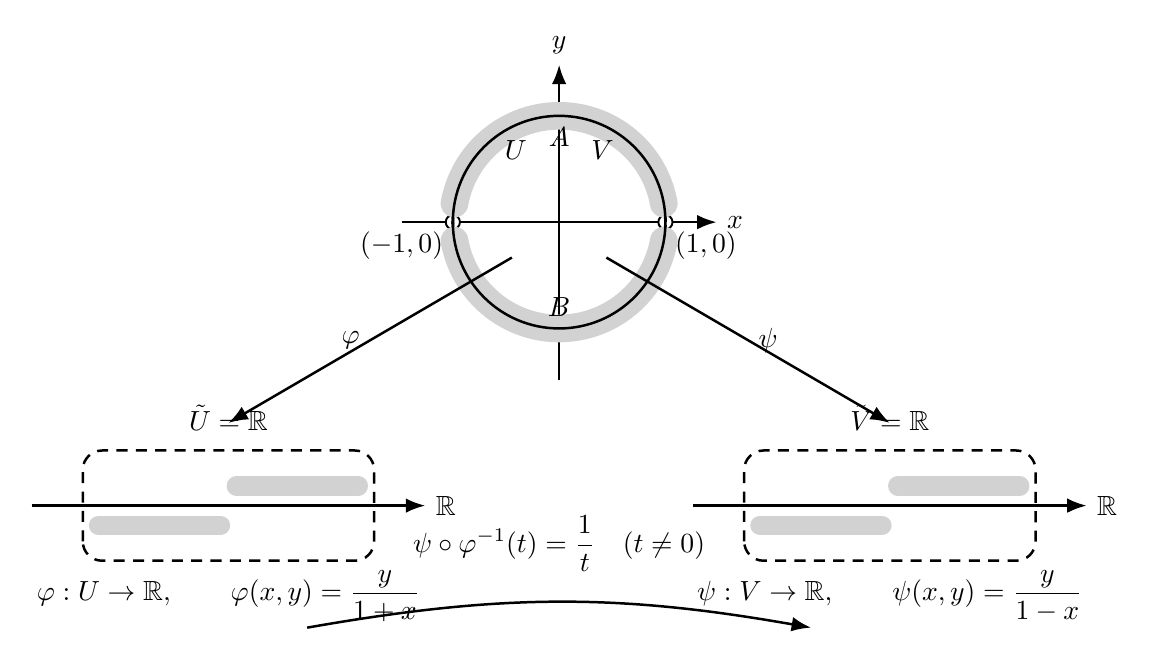
\begin{tikzpicture}[>=Latex,scale=1]
	
	% ------------------------------------------------------------
	% Styles (close to the black/white + gray overlap style)
	% ------------------------------------------------------------
	\tikzset{
		s1/.style={line width=0.9pt},
		Ustyle/.style={line width=1.0pt,dashed,dash pattern=on 4pt off 3pt},
		Vstyle/.style={line width=1.0pt,dashed,dash pattern=on 4pt off 3pt},
		overlap/.style={line width=10pt,draw=gray!35,line cap=round},
		hole/.style={fill=white,draw=black,line width=0.7pt},
		axis/.style={->,line width=0.9pt},
		box/.style={draw=black,dashed,dash pattern=on 4pt off 3pt,
			line width=0.9pt,rounded corners=7pt},
		downarr/.style={->,line width=0.9pt},
		trans/.style={->,line width=0.9pt},
		grayseg/.style={line width=7pt,draw=gray!35,line cap=round}
	}
	
	% ============================================================
	% TOP: S^1 \subset R^2 with U, V, and U\cap V = A \sqcup B
	% ============================================================
	\begin{scope}[shift={(0,3.6)}]
		\def\r{1.35}
		
		% Coordinate axes in R^2 (comment out if you want a cleaner look)
		\draw[axis] (-2.0,0) -- (2.0,0) node[right] {$x$};
		\draw[axis] (0,-2.0) -- (0,2.0) node[above] {$y$};
		
		% Circle S^1
		\draw[s1] (0,0) circle (\r);
		
		% Concrete points (-1,0), (1,0) on this drawn circle
		\coordinate (mone) at (-\r,0);
		\coordinate (pone) at ( \r,0);
		
		% Labels
		\node[below left]  at (mone) {$(-1,0)$};
		\node[below right] at (pone) {$(1,0)$};
		
		% "Removed points" as holes
		\draw[hole] (mone) circle (0.09);
		\draw[hole] (pone) circle (0.09);
		
		% U = S^1 \ {(-1,0)} : dashed circle with small gap at 180 degrees
		\draw[Ustyle] (175:\r) arc (175:360:\r);
		\draw[Ustyle] (0:\r)   arc (0:5:\r);
		
		% V = S^1 \ {(1,0)} : dashed circle with small gap at 0 degrees
		\draw[Vstyle] (5:\r)    arc (5:180:\r);
		\draw[Vstyle] (180:\r)  arc (180:355:\r);
		
		% Overlap U\cap V = S^1 \ {(-1,0),(1,0)} has two components:
		% A (upper arc) and B (lower arc), shaded thick gray.
		\draw[overlap] (10:\r)  arc (10:170:\r);    % A
		\draw[overlap] (190:\r) arc (190:350:\r);   % B
		
		% Redraw circle for crisp boundary
		\draw[s1] (0,0) circle (\r);
		
		% Labels for sets/components
		\node at (-0.55,0.92) {$U$};
		\node at ( 0.55,0.92) {$V$};
		\node at (0, 1.08) {$A$};
		\node at (0,-1.08) {$B$};
		
		% Anchors for arrows to charts
		\coordinate (uAnchor) at (-0.60,-0.45);
		\coordinate (vAnchor) at ( 0.60,-0.45);
	\end{scope}
	
	% ============================================================
	% BOTTOM LEFT: (\tilde U, \varphi) with explicit stereographic formula
	%   \varphi(x,y) = y/(1+x)  (projection from (-1,0) to x=0 \cong R)
	% ============================================================
	\begin{scope}[shift={(-4.2,0)}]
		% Real line axis
		\draw[axis] (-2.5,0) -- (2.5,0) node[right] {$\mathbb R$};
		
		% Dashed rounded rectangle indicating chart domain (schematic)
		\draw[box] (-1.85,-0.70) rectangle (1.85,0.70);
		\node[above] at (0,0.83) {$\tilde U=\mathbb R$};
		
		% Two components of overlap in coordinates (A maps to (0,∞), B to (-∞,0))
		\draw[grayseg] (0.10,0.25) -- (1.65,0.25);     % image of A
		\draw[grayseg] (-1.65,-0.25) -- (-0.10,-0.25); % image of B
		
		% Formula label
		\node[align=center] at (0,-1.15)
		{$\displaystyle \varphi:U\to\mathbb R,\qquad \varphi(x,y)=\frac{y}{1+x}$};
	\end{scope}
	
	% ============================================================
	% BOTTOM RIGHT: (\tilde V, \psi) with explicit stereographic formula
	%   \psi(x,y) = y/(1-x)  (projection from (1,0) to x=0 \cong R)
	% ============================================================
	\begin{scope}[shift={(4.2,0)}]
		% Real line axis
		\draw[axis] (-2.5,0) -- (2.5,0) node[right] {$\mathbb R$};
		
		% Dashed rounded rectangle indicating chart domain (schematic)
		\draw[box] (-1.85,-0.70) rectangle (1.85,0.70);
		\node[above] at (0,0.83) {$\tilde V=\mathbb R$};
		
		% Two components of overlap in coordinates
		\draw[grayseg] (0.10,0.25) -- (1.65,0.25);     % image of A
		\draw[grayseg] (-1.65,-0.25) -- (-0.10,-0.25); % image of B
		
		% Formula label
		\node[align=center] at (0,-1.15)
		{$\displaystyle \psi:V\to\mathbb R,\qquad \psi(x,y)=\frac{y}{1-x}$};
	\end{scope}
	
	% ============================================================
	% Arrows from S^1 down to the charts + transition map
	% ============================================================
	\draw[downarr] ($(0,3.6)+(-0.60,-0.45)$) -- (-4.2,1.05)
	node[midway,left] {$\varphi$};
	
	\draw[downarr] ($(0,3.6)+( 0.60,-0.45)$) -- ( 4.2,1.05)
	node[midway,right] {$\psi$};
	
	% Transition map on overlap in coordinates:
	%   (\psi \circ \varphi^{-1})(t) = 1/t  on  R\setminus{0}.
	\draw[trans] (-3.2,-1.55) to[bend left=10] (3.2,-1.55)
	node[midway,below] {$\displaystyle \psi\circ\varphi^{-1}(t)=\frac{1}{t}\quad (t\neq 0)$};
	
\end{tikzpicture}

\end{document}
